\vspace{-10pt}
\section{Support for Large Number of Streams Using Internal Streams}
\label{sec:internal}
\vspace{-5pt}
As explained in Section 2.2, the number of streams is restricted to a small number 
because of the practical limits on the backup power capacity and the size of fast memory.  
Since the number of supported streams critically impacts the overall performance 
of multi-streamed SSDs, in this section, we propose a new type of streams, 
called {\it internal streams}, which can be
supported without affecting the capacity of a backup power as well as 
the size of fast memory in SSDs.   
Internal streams, which are restricted to be used only for garbage collection, 
significantly improve the efficiency of PC-based stream allocation,
especially when PCs show large lifetime variances in their data lifetime
distributions.

\vspace{-10pt}
\subsection{Program Contexts with Large Lifetime Variances}
\vspace{-5pt}
For most PCs, their lifetime distributions tend to have small variances
(e.g., Figs.~\ref{fig:types_and_PCs}(a), ~\ref{fig:types_and_PCs}(d), and
~\ref{fig:types_and_PCs}(f)).
However, we observed that 
it is inevitable to have a few PCs with large lifetime variances 
because of several practical reasons.
For example, when multiple I/O contexts are covered by the same execution path, 
the corresponding PC may represent several I/O contexts whose data lifetimes are quite different.   
Such a case occurs, for example, 
in the compaction job of RocksDB.
RocksDB maintains
several levels, L1, ..., L$n$, in the persistent storage, except for L0 (or a
memtable) stored in DRAM.  Once one level, say L2, becomes full, all the data
in L2 is compacted to a lower level, i.e., L3.  It involves moving data from L2
to L3, along with the deletion of the old data in L2.  In the
LSM tree~\cite{LSM}, a higher level is smaller than a lower level 
(i.e., the size of (L2) $<$ the size of (L3)). 
Thus, data stored in a higher level is invalidated more frequently than those kept
in lower levels, thereby having shorter lifetimes.

%Once the L1 becomes full,
%\textit{all} the data kept in the L1 are moved to the L2 by the compaction
%module.  The same operation is applied to the other levels (i.e., L3, ...,
%L$n-1$).  The compaction involves reading and writing data from a higher level
%(e.g., L1) to a lower level (e.g., L2).  The data in a higher level (e.g., L1)
%is then removed.  

%While the program context can be used as a useful indicator that determines the
%lifetime of data, we also observe that the same PC could generate data 
%with diverged lifetimes. One of the representative examples is the compaction
%module of RocksDB. RocksDB maintains several levels, L1, ..., L$n$, in the
%persistent storage, except for L0 (or a memtable) stored in DRAM.  Data flushed
%from the memtable are first written to the L1.  Once the L1 becomes full,
%\textit{all} the data kept in the L1 are moved to the L2 by the compaction
%module.  The same operation is applied to the other levels (i.e., L3, ...,
%L$n-1$).  The compaction involves reading and writing data from a higher level
%(e.g., L1) to a lower level (e.g., L2).  The data in a higher level (e.g., L1)
%is then removed.  In the LSM-tree, a higher level is smaller than a lower
%level. Thus, data stored in a higher level is invalidated sooner than data kept
%in lower levels, thereby having much shorter lifetimes.

\begin{figure}[!t]
\centering
\subfloat[RocksDB: L2 Compaction]{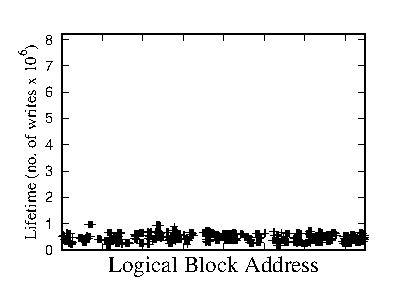
\includegraphics[width=0.19\textwidth]{figure/type_4_new.eps}}  % data from 4/03040047
	\hspace{10pt}
\subfloat[RocksDB: L4 Compaction]{\includegraphics[width=0.19\textwidth]{figure/type_6_new.eps}}
%\caption{The lifetime distribution of the compaction activity.} 
	\vspace{-8pt}
\caption{Lifetime distributions of the compaction activity at different levels.} %shane part
\label{fig:compaction}
	\vspace{-15pt}
\end{figure}




Unfortunately, in the current RocksDB implementation, the compaction step is supported 
by the same execution path (i.e., the same PC) regardless of the level.
Therefore, the PC for the compaction activity cannot effectively separate data with 
short lifetimes from one with long lifetimes.
Fig.~\ref{fig:compaction}(a) and ~\ref{fig:compaction}(b) show
distinctly different lifetime distributions based on the level of compaction:
data written from the level 4 have a large lifetime variance while data written from
the level 2 have a small lifetime variance.

Similarly, in SQLite and GCC, program contexts with large lifetime variations
are also observed.
Fig.~\ref{fig:types_and_PCs}(e) shows large lifetime variances of data files in
SQLite.
Since client request patterns will decide how SQLite updates its tables, 
the lifetime of data from the updating activity of SQLite is distributed 
with a large variance.  Similarly, the lifetime of
data from the outputting temporary files of GCC can significantly fluctuate 
as well depending on when the next compile step starts.   
Fig.~\ref{fig:types_and_PCs}(g) shows long lifetimes of 
object files/executable files after 
a Linux build was completed
(with no more re-compilling jobs).
However, the lifetime of the same object files/executable files 
may become short when if we have to restart the same
compile step right after the previous one is finished
(e.g., because of code changes).

For these {\it outlier} PCs with large lifetime variations, 
it is a challenge to allocate streams in an efficient fashion unless 
there are more application-specific hints (e.g., the compaction level in
RocksDB) are available.  
As an ad-hoc (but effective) solution, when a PC shows a large variance 
in its data lifetime, we allocate an additional stream, called an internal stream, 
to the PC so that
the data written from the PC can be better separated between the original 
stream and its internal stream.  
In order to support internal streams, the total number of streams may 
need to be doubled so
that each stream can be associated with its internal stream.

\vspace{-10pt}
\subsection{Efficient Implementation of Internal Streams}
\vspace{-5pt}
As described in Section 2.2, it is difficult to increase the number of 
(normal) streams.  However, 
if we restrict that internal streams are used only for data movements
during GC,
they can be quite efficiently
implemented without the constraints on the backup power capacity and fast memory size.  
The key difference in the implementation overhead between normal streams and 
internal streams comes from a simple observation that data copied during 
GC do not need the same reliability and performance support as for host writes.  
Unlike buffered data from host write requests, valid pages in
the source block during garbage collection have no risk of losing their data 
from the sudden power-off conditions because the original valid pages are always available.    
Therefore, even if the
number of internal streams increases, unlike normal streams, 
no higher-capacity backup capacitor is necessary for managing buffered data for internal streams. 

The fast memory requirement is also not directly increased as the number 
of internal streams increases.   
Since internal streams are used only for GC and most GC can be handled as background tasks,
internal streams has a less stringent performance requirement.  
Therefore, data structures for supporting internal streams can be placed 
on DRAM without much performance issues.  
Furthermore, for a read request, there is no need to check if a read request 
can be served by buffered data as in normal streams because the source block always 
has the most up-to-date data.  
This, in turn, allows data structures for internal streams to be located in slow memory.
Once an SSD reaches the fully saturated condition where host writes and GC 
are concurrently performed, the performance of GC may degrade a little because of
the slow DRAM used for internal streams.   
However, in our evaluation, such cases were rarely observed under a 
reasonable overprovisioning storage capacity.

\begin{comment}
{\color{blue}
With regard to power resources, the buffering mechanism can be used for internal streams to maximize flash parallelism, but there is a big difference that no power resource is required to guarantee data integrity of buffered data.
Buffered data of host write will be lost if the data is not stored during power off handling.
However, the buffered data of internal migration doesn't need to be saved during power off handling. Because the original data always exists in the source block of migration. 
Therefore, there is no problem in ensuring data integrity without special handling or power resource requirement.

Unlike external streams, which require host requests to be handled directly in the foreground,
internal streams can be handled as background operations, 
so even if the data structures of internal streams are located in relatively slow memory, 
host request processing performance may not suffer. 
And the data structures for internal streams do not need to be checked during 
read request processing.
This is due to the fact that the data managed by the internal stream is not up-to-date 
and the source block has the same data. 
So read performance is not affected by usage of slow memeory for internal streams.
Under saturated conditions, which require concurrent processing of GC while processing a host write request, 
performance degradation may occur if slower memory is used in the internal stream, but performance degradation is small compared to using slow memory for external streams.
}
\end{comment}




